\documentclass[12pt]{article}
% $Id: bioperl-article.tex,v 1.16.2.1 2002-04-06 23:34:05 lapp Exp $
% $Log: not supported by cvs2svn $
% Revision 1.16  2002/04/06 19:07:08  lapp
% Spelled out GNF.
%
% Revision 1.15  2002/04/05 23:15:32  jason
% some changes to format towards GR - a few sentance reworks and transitions - cut it down to 5 main topics, pages for weblinks and each figure with captions
%
% Revision 1.14  2002/04/05 17:19:02  jason
% grammatical changes
%
% Revision 1.13  2002/04/02 00:07:13  jason
% rework, with Mark's comments - still need to add Matt's suggestions
%
% Revision 1.12  2002/03/25 14:17:28  jason
% small TeX bugs
%
% Revision 1.11  2002/03/24 20:49:13  jason
% reworking abstract, removed redundancy and greatly simplified the interoperability section.  Need to condense to probably 4-5 main sections
%
% Revision 1.10  2002/03/21 21:50:04  jason
% reworked abstract for GR and moved examples around.  Reworked abstract for GR and moved examples around.  Added statistics about tests and number of modulesTable for Modules rather than list.
%
% Revision 1.9  2002/03/19 10:58:47  heikki
% fixing examples, lot's of typos in the docs, minor changes
%
% Revision 1.8  2002/03/13 21:21:08  jason
% 3rd draft - with Lincoln's changes
%
% Revision 1.7  2002/03/04 22:18:09  jason
% Some reworking of text, placeholders for expansion on the major 
% theme of open-source developmentmore references and testing out 
% the lstlisting for code section, lines
% are not wrapping nicely though in 2-column mode with the code,
% Author list still incomplete and need to move acknowledgements
% around some more
%

\usepackage {listings,hyperref,url,apalike,layouts,
	     	epsfig,graphicx,keyval,fancyhdr,
	     setspace,fullpage }

\begin{document}

\doublespacing
%%>HL I'd suggest a different title.
\title{The Bioperl Toolkit: Perl Modules for the Life Sciences}
\author{Jason E Stajich$^1$ \and
Hilmar Lapp$^2$ \and
Heikki Lehv\"{a}slaiho$^3$ \and 
Lincoln D Stein$^4$ \and Ewan Birney$^3$ \and
Bioperl Project Team \thanks{Bioperl Mailing List bioperl-l@bioperl.org} \\
$^1$ \small{\textit{University Program in Genetics, Duke University,  Durham, NC USA}} \\
$^2$ \small{\textit{Genomics Institute of the Novartis Research
Foundation (GNF), San Diego, CA USA}} \\
$^3$ \small{\textit{European Bioinformatics Institute, Welcome Trust
Genome Campus, Hinxton, Cambridge UK}} \\
$^4$ \small{\textit{Cold Spring Harbor Laboratories, Cold Spring Harbor, NY USA }}\\
}
\maketitle
\begin{abstract}

The Bioperl project is an international open source collaboration of
biologists, bioinformaticians, and computer scientists that has
evolved over the last 7 years into the most comprehensive library of
%%<HL changed order of managing and manipulating
Perl modules for managing and manipulating life science information.
Bioperl provides an easy-to-use, stable, and consistent programming
%%<HL inserted Bioperl
interface for bioinformatics application programmers.  The Bioperl
modules has been successfully and repeatedly used to achieve otherwise
complex tasks with only a few lines of code.  The Bioperl object model
has been proven to be flexible enough to support enterprise-level
applications such as EnsEMBL, while at the same time keeping an easy
learning curve for novice Perl programmers.  Bioperl is also capable
of interoperating with other programming languages like Python and
Java through the evolving BioCORBA bridge. 
%%!HL Changed the next sentence. May not be the best suggestion either.
Furthermore, Bioperl provides access to a common data storage by fully
supporting the evolving BioSQL and Open Bioinformatics Database Access
projects. 
%%!HL I feel this needs to be changed. We're not publishing this as an
%%!HL open advertisement of open source, it's rather an implicit ad. GR is
%%!HL not a software engineering journal.
%%!HL Better suited here would be to say briefly what this paper will
%%!HL tell about Bioperl.
The successful development of Bioperl depended in a large
part on the open source nature of the project. We outline how this
approach is a valuable mechanism for collaborative projects.

[ Bioperl is available as open source software free of charge and
licensed under the Perl artistic license at \url{http://www.bioperl.org/}. ]

\textbf{Contact:} Bioperl project list \url{bioperl-l@bioperl.org}.

\end{abstract}

\section{Introduction}

Computational analysis is an integral part of modern biological
research.  Numerous computer software tools exist to perform 
data analyses, but it is not simple to automatically
combine data and results from multiple sources without the use of
computer software designed to read and write data specific to the
biological domain.  
%%!HL I feel this statement is too broad, as it probably doesn't apply
%%!HL to algorithm research labs.
Bioinformatics consists largely of applying a
particular logic to this data integration.

%%<HL Changed wording slightly.
The programming language Perl \cite{perlref} is by far the most widely used
programming language for these tasks, and is commonly thought of as
the language most easily grasped by newcomers to the field.  Perl has
been extremely successful for connecting software applications together into
sequence analysis pipelines, converting file formats, and extracting
information from the output of analysis programs and other text files.

Much of the Perl software in bioinformatics is specific to a
%%!HL general->generic
particular lab or institution and is not written in a generic way so
%%!HL added 'too'
that it can be used by others, too.  The Bioperl toolkit brings
together reusable Perl modules containing generalized routines
specific to biological and life science information.  A primary
motivation behind writing the toolkit is the authors' desire to focus
%%>HL one->a
energies on a solution whose components could be shared rather than
%%<HL In our minds->The idea is
duplicating effort.  The idea is once a routine is written for
parsing and interpreting sequence from EMBL and Genbank format
sequence files, no one else should have to worry about writing their
own.  In this spirit we chose to make our code freely available and
%%>HL Inserted open-source ref. Inserted 'and improvements'.
Open Source \cite{open-sourc-ref} so that others could contribute
their solutions and improvements to the project as well.  Just as the
Human Genome Project was speeded and made more efficient by public
sharing of data, so has the open nature of the Bioperl project reduced
the time for solutions and new tools to reach the community
\cite{waterston}.

However, to be adopted by the community our software has to be user
%%!HL we've -> we have
friendly.  To that end we have both provided extensive documentation of
all the methods in each module, a graphical diagram of the objects in
the toolkit, and tutorials with examples of common problems.
Additionally we have written a module named Bio::Perl which provides
simple methods such as \textit{read\_sequence} which reads a sequence
from a file for users who do not want to study the entire module
%%!HL their -> her
hierarchy.  The goal of Bioperl is to help a user focus on her
%%>HL process -> filter, and according changes
specific problem at hand, such as the logic needed to filter hits in a
%%!HL on than -> than on
BLAST \cite{blast} report by certain criteria, rather than on the
actual mechanics of \textit{parsing} that BLAST report.

\section{Methods}

%%<HL inserted 'at a time'
The Bioperl project began in 1995 \cite{chervitz-bits} at a time when
there were few programming toolkits for manipulating biological data
or results from sequence analysis programs.  Although Perl had already
gained widespread popularity in the bioinformatics community for its
efficient support of text processing and pattern matching tasks, there
were in fact no biological toolkits available in this language.

The project grew out of the following observations.  
\begin{itemize}

\item First, even though file formats of different analysis programs
are different, the information they represent is the same.  For
example, a pair-wise alignment is always between two sequences and has
common properties such as length, score, fraction of identities, start
and end of the aligned sequences, and so forth.

\item Second, the number of data structures needed to represent
information flow is limited, and common to most applications, such as
%%<HL small -> limited
sequences, annotation, features, and alignments.  This permits a limited
%%!HL inserted 'a'
set of modules to be reused for a variety of purposes.
%%>HL I'd leave this out. To me it doesn't make the argument any
%%>HL stronger, and in fact there is a hierarchy that is confusing to some.
%and avoids creating a confusing hierarchy of components.

%%>HL changed order of words, it wasn't clear enough for me before
\item Third, there is a common set of operations performed on these
%%>HL inserted 'operations, for example,'
data structures.  These operations, for example, include reading and
writing information to a file, querying a sequence for its features,
and translating a coding sequence into protein.

\end{itemize}

This scenario naturally lends itself to the principle of
object-oriented programming, which Perl emulates with modules.
%%>HL changed wording of the next two sentences
Object-oriented programming is the practice of encapsulating abstract
data types and operations on these data types as logical and broadly
applicable components. For instance, a DNA Sequence component would
contain methods such as retrieve the accession number, reverse
complement the sequence, or translate to a protein sequence.

%%<HL started a new paragraph
The mission of Bioperl is to provide an easy-to-use object-oriented
Perl library that contains data structures and operations commonly
%%!HL corrected typo
used in the life sciences as clean, generic, and re-usable modules.
By separating the components into logical groups, such as sequences,
alignments, and databases, we have been able to add features to a
specific module without necessarily affecting the rest of the toolkit
%%>HL component->aspect (avoids using the term in multiple meanings)
library.  This separation is a key aspect of object-oriented
%%>HL changed last part of the sentence to mention stability (as this
%%>HL is the thing coming through separation)
programming and permits us to produce generic components with a stable
interface for the programmer (API).

%%>HL objects->components to stay consistent in language
At present the components and operations in Bioperl center around
biological sequence analysis and annotation.  In the last year the
project has expanded to address new areas including phylogenetics,
maps, protein structure, and bibliographic references.  The project
has over 300 modules and comprises more than 160,000 lines of code and
embedded documentation.  The Perl modules are organized by logical
names so that, for example, the Bio::Search hierarchy contains modules
related to database searches and Bio::Graphics contains modules that
are related to drawing.

When designing Bioperl objects our objective was to provide a
programming interface that is very easy to use but that at the same
time could be easily extended in its capabilities and behavior through
code reuse.  Using an object-oriented paradigm we followed certain
design principles.

\begin{itemize}

\item Separating the interface from the implementation.  The key
%%!HL removed object. Either it's an object or a class, not both.
information about a class is the names of its public methods and their
list
%%>HL Added the ref to Java for better understandability
of accepted arguments.  Similar in concept to interfaces in Java, we
built interfaces as collections of methods which describe the expected
behavior of a module, but do not do any of the work.  Child classes
%%>HL changed wording
implement the interfaces, providing specializations of their
%%>HL inserted comma
parents to perform specific tasks.  
%%>HL the following I think isn't the best example; SeqIO isn't a true
%%>HL interface either. It's a factory, and the design pattern is a
%%>HL strategy pattern. It could be an example for which patterns are used
%%>HL in the design.
For example, the sequence parsing factory class Bio::SeqIO describes
methods \textit{next\_seq} and \textit{write\_seq} which are
implemented differently by the child classes Bio::SeqIO::genbank and
Bio::SeqIO::embl for reading and writing their specific sequence data
format.

%%>HL changed second part of sentence. Also, changed a lot more of the
%%>HL whole paragraph.
\item Generalize common routines into a single module providing a base
framework for the respective operations.  As an example, we
centralized basic data Input/Output (IO) operations into IO object,
called Bio::Root::IO. Because all modules that need IO data access use
operations from the IO module, these operations are implemented across
the entire package in a consistent way. This design choice also
provides for single points of fixing and enhancing functionality.
%%>HL I don't feel this is so important that we need to substantiate
%%>HL it with a figure. MHO.
Figure 1 shows a schematic view of how 2 modules which have different
tasks inherit from a single IO module which provides a function that
is shared.

\end{itemize}

In Bioperl we followed these two design patterns \cite{gangoffour}
wherever possible.  To help distinguish implementation classes from
interface definition we used a capital 'I' appended to the module
%%>HL changed wording of the next sentence.
name. As an example, the interface for a full-featured sequence object
is defined in Bio::SeqI, and the implementing class is named Bio::Seq.

Bioperl is written purely in Perl and depends on at least version
%%>HL added the current version to relate 5.005 to. 5.6.1 may not be
%%>HL correct though.
5.005 of the Perl interpreter (the current stable version of Perl as
of the time of writing is 5.6.1).  The toolkit has been checked for
cross-platform compatibility on most UNIX and UNIX-like operating
%%<HL started new sentence. Changed wording slightly.
systems.  In addition, Bioperl has been tested and runs on the
Macintosh OS X as well as Microsoft Windows operating systems.  Since
the toolkit is run through the Perl interpreter, specific issues are
often due to compatibility between different versions of Perl.
%%>HL added operating system-. Changed bugs->problems.
Descriptions of operating system-specific problems and their solutions
are available from the Bioperl website.

In addition to pure Perl solutions to bioinformatics problems, Bioperl
can take advantage of external data analysis packages.  Currently the
toolkit supports interactions with applications in the EMBOSS
\cite{emboss} suite, NCBI BLAST, and the multiple sequence alignment
programs ClustalW \cite{clustalw} and T-Coffee \cite{tcoffee}.  In
some cases, when an external package is not available, Bioperl will
fall back to using a slower method, either by emulating the package in
pure Perl or by invoking a network-based analysis service such as the
NCBI BLAST analysis queue.  Additional work is in progress to
incorporate into the project access to remote analysis services at the
%%>HL shouldn't there be locations of these institutes?
European Bioinformatics Institute and Pasteur Institute.

In order for us to produce fairly uniform software code we established
%%<HL good->widely accepted. Added 'styles' at the end.
coding guidelines that are extensions of widely accepted
object-oriented
%%>HL were->are
programming styles.  All modules are required to meet minimal
%%>HL releasing->release, included->include
standards before release.  These standards include a complete set
of regression tests, well-formed embedded documentation for each
method, and concise example code in the SYNOPSIS section of each
%%>HL passive speech->active speech
module's documention.  We use the Perl embedded documentation format (called
POD, or Plain Old Documentation) to provide annotation within
the source code.  This documentation can be converted to text, TeX, or
HTML.  We have used the Pdoc \url{http://pdoc.sourceforge.net} tool to
%%>HL organized->easily navigable
generate colored and easily navigable documention in HTML for easy online
browsing.

%%>HL Added 'and comprehensive unit-'
The development process involves integrated and comprehensive unit-testing
of the code.  We
%%!HL insuring->ensuring
accomplished this by ensuring that each module has a test in the
Bioperl test system.
%%>HL I feel the digression on XP is not very appropriate here; it
%%>HL doesn't add value. Rather, one could refer the reader to XP
%%>HL literature for more about unit testing and its advantages.
% This approach is effective in locating newly introduced bugs and is a
% tenent of the Extreme Programming\cite{xprogramming} methodology.  The
% Extreme Programming approach is to build the test for a module first
% and implement the module which completes the test second.  This
% approach insures that all tested aspects of the module's
% implementation were correctly completed successfully. 
The Bioperl 1.0 release has over 3000 such tests that the code had to
pass.
% which assists in insuring the quality of the source code releases and
% checks that new changes to the code do not break the expected behavior
% of modules.

%%>HL reworked this paragraph almost completely.
To support multiple developers in different time zones and
institutions, the entire Bioperl source code is hosted by the Open
Bioinformatics Foundation (OBF) \cite{obf-ref} on a CVS server. CVS
stands for Concurrent Version Control system
(\url{http://www.cvshome.org}) \cite{cvsbook} and allows multiple
developers to on the software source code concurrently without having
to coordinate every single change.  The ability to share code easily
and quickly has shown itself to be key for establishing a successful
open source project. OBF also hosts the Bioperl website at
http://www.bioperl.org/.

\section{Results}

Bioperl has 10 active developers led by a core of 5 primary developers
%%!HL insure->ensure
who ensure that standards are met, prepare code releases, and set the
vision for the project.  The mailing lists for the project include
%%>HL started new sentence. Changed wording.
1300 subscribers. As of this year, the website has seen about 10,000
unique visitors each month.  The project has been used in a variety of
endeavors including genome sequencing, annotation, sequence variation
elucidation, disease gene discovery, and comparative genomics.

By far the most advanced use of the Bioperl toolkit has come through
the EnsEMBL\cite{ensembl-nar} project.  The basic sequence handling,
file format parsing, and sequence features for annotation model have
been used as building blocks for automatically annotating the
\textit{Danio rerio}, \textit{Drosophila melanogastor}, \textit{Fugu
rubripes}, \textit{Homo sapiens}, and \textit{Mus musculus} genomes
(\url{http://www.ensembl.org}).

%%>HL changed wording
Additionally, the Genquire\cite{genquire} annotation package builds on
top of the Bioperl object model and stores sequence and annotation
%%>HL removed persistent and model. What is a non-persistent database?
%%>HL Also, you cannot physically store anything in a database model.
data in a database.  The sequence rendering capabilities are
partitioned into a specific Bioperl package called bioperl-gui. 
%%>HL is the following really important to Bioperl's cause?
The database model used by Genquire has been updated to utilize the
Open Bioinformatics Database Access (OBDA)
(\url{http://obda.open-bio.org}) sequence database design, which will
allow the other OBF toolkits to access data written by the Genquire
system.

The Generic Model Organism Browser (GMOD) \cite{gmod}, Distributed
Annotation System Perl (DAS) server \cite{das}, and TFBS
\cite{tfbs} all use the Bioperl object model to describe sequences and
Bioperl tools to complete analyses.  The GMOD system is a web
interface to databases of features for a genome project.  The DAS
system provides researchers a means to locally annotate sequences and
publish the annotations to the community via the DAS XML protocol.
TFBS provides a perl implementation of objects for DNA sequence pattern
representation by matrix profiles, with associated methods for searching
the sequences for the occurence of patterns, pattern storage, and
generation of new patterns. The implementation uses Bioperl sequence,
alignment, sequence feature and feature pair objects.

\subsection{Interoperability}

%%>HL almost completely rewrote this section. To me, it's still too
%%>HL long and should be cut to theh juicy bits in order not to lose focus
Bioinformaticists are often faced with the situation that basically
almost all of the individual pieces necessary to construct a good
solution to a problem are already available, but they have been
written in different programming languages such as C, Java, and
Python. The ability to re-use those pieces in such a situation
critically depends on the interoperability of the individual software
components.

External executable programs can be used within a Perl script simply
by invoking them (a process often called ``shelling out''). This
mechanism is used in Bioperl, for instance, for interfacing with NCBI
Blast, and the entire EMBOSS suite of analysis programs. 

Some of external programs require that data be available in a certain
format or within a certain database.  Part of the mission of Bioperl
is to support at least the most common and standard formats. As a
trivial example, many analysis programs expect sequences in FASTA
format, which can be easily written from any other sequence format in
Bioperl. Less trivial, Bioperl provides similar interconversion
%%HL FIXME Is this true?
functionality for the most popular multiple sequence alignment
formats. Furthermore, all classes inheriting off
%%HL FIXME or is it Bio::SeqFeatureI?
Bio::SeqFeature::Generic can be dumped to and re-created from GFF, a
standard for exchanging sequence features between programs. In
Bioperl, this capability not only extends to the entire heirarchy of
gene structure classes, but also to databank search results (`hits').

Recently, Bioperl started to support from the beginning upcoming
%%HL FIXME there need to be references and the precise name of the classes
standard models for sequence and sequence feature databases. This
means for example that databases compliant with these models can be
populated through scripts using the Bioperl toolkit, and the content
can be visualized through an interactive graphical interface provided by
the Biojava toolkit.

Bioperl also supports a number of Extensible Markup Language (XML)
standard data exchange formats accepted in the Bioinformatics
community. XML provides a means for creating data in a language and
platform independent manner.  Previous work has outlined scenarios
where XML has been useful in a biological context
\cite{xmlbioinformatics}.  XML standards supported by Bioperl include
%%HL FIXME BSML and GAME need to be spelled out and cited
BSML, GAME, NCBI BLAST XML, Medline XML provided by the European
Bioinformatics Institute's Bibliographic Query Service (BQS), and
Entrez Pubmed XML format. Some of these standards are currently only
supported in read-only mode, though.

%%HL FIXME CORBA needs to be cited and the reader referred to that for
%%HL further details.
Software can interoperate with other software not only through the
invocation of external programs, but also through invoking methods on
remote components possibly written in a different programming language
than the calling component.  Hence, such a mechanism constitutes the
tightest integration of re-usable software components in a
language-independent way. The Common Object Request Broker
Architecture (CORBA) provides an architecture for enabling this
%%HL FIXME cite examples
technology, and implementations are available from commercial vendors
(e.g., Borland Inprise) as well as Open Source projects. Bioperl is
compliant with one of the proposed standards for CORBA components for
biological processes, namely the BioCORBA
(\url{http://www.biocorba.org}) project.  BioCORBA is also supported
by the Biojava (\url{http://www.biojava.org}) and Biopython
(\url{http://www.biopython.org}) projects, as well as the Object
Management Group's Life Science Research group
(\url{http://lsr.ebi.ac.uk}). This means that eventually all three
language-specific projects for re-usable software components in
Bioinformatics will be able to fully interoperate.

\section{Conclusions}

In the future, Bioperl will continue to evolve in order to address
more issues in bioinformatics.  We plan to create objects to manage
sequence assembly information, haplotype maps, gene expression, and
protein interaction data.  Additionally, projects focusing on
%%!HL corrected typo
multi-species comparisons are building Perl modules to manage the
%%!HL this needs to be cited, or give examples (fugu?)
alignment and syntenic information.  We are creating software layers
to interact with OBDA databases, developing an analysis pipeline
system to provide automated annotation, and expanding the supported
file formats the toolkit can read and write.

We feel that much of the success of the Bioperl toolkit development
effort can be attributed to the Open Source nature of the
%%<HL effort->project
project which
%%>HL added 'and changing'
has allowed a diverse and changing group of individuals to participate
%%<HL project->effort
in a collaborative effort.  We have successfully encouraged users of
%%>HL changed the second part of the paragraph considerably.
the toolkit to assist in the development by contributing bug fixes,
documentation enhancements, and entirely new functionality for the
benefit of all users.  This and the guiding principle to get working
software written in an extensible manner has made Bioperl an excellent
platform for Perl bioinformatics software development.  The open
sharing and discussion of ideas that embodies the scientific spirit
has thereby proven to be successful in the world of software
development for scientific purposes as well.  Bioperl has grown and
will continue to grow in those directions in which its users grow, as
more often than not Bioperl users are Bioperl developers as well.

\section{Acknowledgements}

The Bioperl Core is Jason Stajich, Hilmar Lapp, Heikki
Lehv\"{a}slaiho, Lincoln Stein, and Ewan Birney.  The project has seen
%%>HL added 'given in alphabetical order'
signifigant contributions from the following people, given in
alphabetical order: David Block, Kris Boulez, Steven Brenner, Brad
Chapman, Steve Chervitz, Michele Clamp, Tony Cox, James Cuff, Chris
Dagdigian, Andrew Dalke, Allen Day, Arne Elofsson, Mark Fiers, Georg
Fuellen, James R Gilbert, Ed Green, Roger Hall, Peter van Heusden,
Joseph Insana, Nicolas Joly, Ian Korf, Aaron J Mackey, Brad Marshall,
Chad Matsalla, Chris Mungall, Emmanuel Mongin, Brian Osborne, Lorenz
Pollak, Matthew Pockock, Todd Richmond, Martin Senger, Peter
Schattner, Elia Stupka, Gert Thijs, Charles Tilford, Andrew Walsh, Kai
Wang, Mark Wilkinson, and Alex Zelensky.

Additional ideas and help came from other OBF project team members
including Jeff Chang, Thomas Down, Keith James, and all of the Bioperl
%%>HL added from whom we stole what
mailing list members. Some parts of the object model, especially
locations, where adopted from the excellent work of the Biojava
project and its leaders Thomas Down and Matthew Pocock.

We would like to especially acknowledge Steve Chervitz for his
previous role as Bioperl project leader.  Special thanks also go to
Brian Osborne and Peter Schattner for their excellent documentation
and tutorial work, and Chris Dagdigian for his tremendous support as
system administrator for the project computers.

The Bioperl project and its sister projects (commonly referred to as
the Bio\{*\} projects) are supported under the umbrella of the Open
Bioinformatics Foundation (OBF) \url{http://www.open-bio.org}.
OBF is supported by hardware donations from Compaq and Sun
Microsystems, and we graciously accept donated bandwith and computer
server space from Wyeth.

J.E.S is supported by an NIH Genetics training grant.  We thank
F.Dietrich, M.DeLong, and M.Hahn for their comments on this manuscript.

\bibliography{bioperl}
\bibliographystyle{apalike} 

\newpage

\section{Website References}

\url{http://www.biocorba.org}, BioCORBA Project. \\
\url{http://www.biojava.org}, Biojava Project. \\
\url{http://www.biopython.org}, Biopython Project. \\
\url{http://www.cvshome.org}, CVS Home Page. \\
\url{http://www.ensembl.org}, EnsEMBL Project Home page. \\
\url{http://obda.open-bio.org}, Open Bioinformatics Data Access. \\
\url{http://www.open-bio.org}, Open Bioinformatics Foundation. \\
\url{http://lsr.ebi.ac.uk}, Object Management Group's Life Science Research group. \\
\url{http://pdoc.sourceforge.net}, Pdoc Home Page. \\
\url{http://forkhead.cgr.ki.se/TFBS/}, TFBS Project. \\

\newpage 

% for right hand top labels

\pagestyle{fancy}
\fancyhf{}
\renewcommand{\headrulewidth}{0pt}

\rhead{Stajich\_Table1}

\begin{table}[h]
\begin{tabular}{|l|l|}
\hline
\textbf{Modules} & \textbf{Description} \\
\hline
Bio::Seq &  Sequences and their properties \\
Bio::SeqIO & Sequence data input/output \\
Bio::Index & Local sequence database indexing and retrieval \\ 
Bio::DB & Remote database access for sequences and references via HTTP \\
Bio::DB::GFF & Local GFF database for DAS and GMOD \\
Bio::SeqFeature & Feature representation and annotation \\
Bio::Annotation & Generic annotation \\
Bio::AlignIO, Bio::SimpleAlign & Multiple alignment representation \\
Bio::LiveSeq, Bio::Variation & Sequence variations and mutations \\
Bio::SearchIO, Bio::Search  & Sequence database searches and their Input/Output \\
Bio::Tools &  Miscellaneous analysis tools \\
Bio::Tools::Run &  Wrapper for executing local and remote analyses \\
Bio::Tree, Bio::TreeIO & Phylogenetic trees and their Input/Output  \\
Bio::Structure & Protein structure data \\
Bio::Map, Bio::MapIO & Biological maps and their Input/Output \\
Bio::Biblio, Bio::DB::Biblio & Biblopraphic References and Database
retrieval \\ 
Bio::Graphics & Graphical displays of sequences \\
\hline
\end{tabular}
\caption{Major Bioperl module groups}
\label{modules}
\end{table}

\newpage

\rhead{Stajich\_Figure1\_caption}

Figure 1.  Object-oriented inheritance of the readline() method to the
Sequence Reader and Report Reader modules from the IO class module
illustrates how shared functions can be aggregated and reused.

\newpage

\rhead{Stajich\_Figure2\_caption}

%%>HL this should clarified as to the format in which the sequence
%%>HL comes down the wire; i.e., the point is you don't worry about the
%%>HL format even though it's EMBL at one time and GenBank if you use GenBank.
Figure 2. Sequence retrieval from the Remote GenBank Database at EMBL.
This code retrieve an mRNA sequences from the EBI EMBL databank with
the accession number U14680 and write the sequence out in GenBank
format to the screen.  One could replace Bio::DB::EMBL with
Bio::DB::GenBank and instead retrieve the sequence from NCBI.

\newpage

\rhead{Stajich\_Figure3\_caption}

Figure 3. BLAST parsing. A BLAST report is parsed and only hits meeting
an e-value and length threshold are saved in the array @HitsToSave.  
In this case any hit with evalue greater than 0.001 or length less 
than 120 residues will be excluded.  Once the list of hits is built 
one can print out the name of each of the Hits which had High Scoring
Pairs (HSPs) that met the criteria

\newpage

\rhead{Stajich\_Figure1}

\centerline{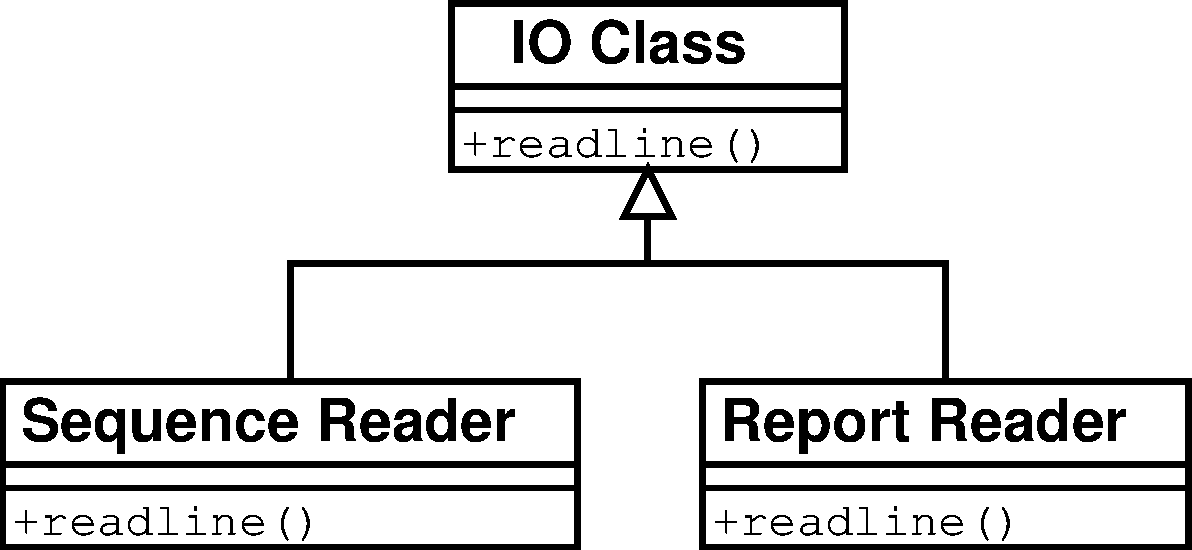
\epsfig{file=oo_inheritance.pdf}}

\newpage

\singlespacing

\rhead{Stajich\_Figure2}

\lstset{
	language=Perl,
	basicstyle=\small,
%	labelstyle=\tiny,
%	labelstep=1,
	stringstyle={} }

\begin{scriptsize}
\begin{lstlisting}{}
use Bio::DB::EMBL;
use Bio::SeqIO;

my $db = new Bio::DB::EMBL();
my $seq = $db->get_Seq_by_acc("U14680");
my $seqout = new Bio::SeqIO(-format => "genbank");
if (defined $seq) { # in case DB doesn't return anything
    $seqout->write_seq($seq);
}
\end{lstlisting}
\end{scriptsize}

% $

\newpage

\rhead{Stajich\_Figure3}
%%>HL I modified the following script fragment to not use a label, and to
%%>HL better follow a naming convention. HL
\begin{scriptsize}
\begin{lstlisting}{}
use Bio::SearchIO;
# Let's parse a BLAST report 
my $search = new Bio::SearchIO(-format => 'blast',
          		       -file   => 'report.bls');
my @hitsToSave;
my $cutoff_Evalue = 0.001; # max e-value is 0.001
my $cutoff_Len   = 120;    # min length of 120 residues
while(my $result = $search->next_result) {
  while(my $hit = $result->next_hit) {
    while( my $hsp = $hit->next_hsp ) {
      if( $hsp->evalue < $cutoff_Evalue && 
	$hsp->length('total') >= $cutofflen ) { 
	push @HitsToSave, $hit;
	last;
      } 
    }
  }
}
# process hits that meet criteria
print "Hits:\n";
foreach my $hit ( @hitsToSave ) {
  print $hit->name, "\n";	
}

\end{lstlisting}
\end{scriptsize}

\end{document}
